\documentclass[12pt]{article}

\usepackage[vmargin=25mm, hmargin=20mm]{geometry}
\usepackage{parskip}
\usepackage{graphicx}
\usepackage{minted}
\usepackage{booktabs}
\usepackage{subcaption}
\graphicspath{ {../figures/} }

\begin{document}
\title{Hash Table Performance}
\author{Ben Ellis}
\date{\today}
\maketitle

\section*{Introduction}
% Decided to implement chained (and possibly open addressed) hash table.
% Investigate effects of these choices on the read and write performance
In this report I present an investigation into different implementations of
a hash set which stores unsigned 32 bit integers. 

A hash set stores integers by using a hash function, $h$, to compute an index
into an array from the input and then storing the element in that location. 
In the case of two elements mapping to the same location, called a conflict, there are two main
courses of action. The first is to continue probing other indices in the array until
a free slot is found, and the second is to extend the array into an array of linked lists, and
attach the element at a free slot later in the table. This form of hash table is illustrated in
Figure~\ref{fig:chaining}.

% Explain how a chained and open-addressed hash table works
\begin{figure}
    \centering
    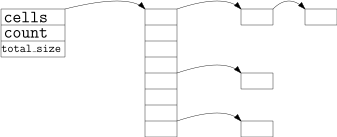
\includegraphics[width=0.5\textwidth]{chained_table}
    \caption{Diagram illustrating a chained hash table}\label{fig:chaining}
\end{figure}

\section*{Implementations And Analysis}

I started by implementing a simple hash table with collision resolution via chaining. 
The definitions for the structs required are shown in Listing~\ref{fig:def}. Notice that
the table contains a pointer to a pointer to a value, that is there must be 2 memory 
references (and potentially two cache misses) before a value can be accessed. This is a
disadvantage compared to open addressing where the values are stored directly in the table.
The major advantage of this form of hash table is that deleting does not waste space.
\begin{listing}
    \centering
    \begin{minipage}[t]{.5\textwidth}
    \begin{minted}{C}
    typedef struct CELL {
        struct CELL *next;
        uint32_t val;
    } cell_t;
    typedef struct TABLE {
        uint32_t count;
        uint32_t total_size;
        cell_t **cells;
    } table_t;
    
    table_t *create_table();
    void insert(table_t *, const uint32_t);
    bool contains(table_t *, const uint32_t);
\end{minted}
\end{minipage}
\caption{Code for the initial definition of the chained hash table. The next pointer is listed first in the cell\_t
type so that no padding is added.}
\label{fig:def}
\end{listing}

Inserting into the table is done by hashing the integer to find the index at which to insert it, and following the linked
list to the end before adding a new cell there. Checking a value is present in the table follows a similar process, but
checks for the presence of the value rather than inserting a new one. The only wrinkle is resizing the table. When the 
table reaches above a certain occupancy, it is doubled in size to retain performance. This is done by finding the 
correct index in the new table at which to insert the new value, and copying the cell to the end of the linked list.

I implemented a few simple tests to benchmark the performance of this data structure. The first inserted the integers
in the range $[0, 10^7)$ in order into the table, and then read them out in order. The results are shown in the 
Ordered Write and Ordered Read columns of Table~\ref{tab:perf} respectively. The second set of tests inserts some random
numbers into the table and reads either one of these numbers or a random number. The choice of whether to read a number 
that is in the table or one that is likely not is chosen at random. One test of this type inserts $256$ integers 
and reads $10^7$ times, and the other does the opposite, writing $10^7$ integers and reading $256$ times. These are 
listed in Table~\ref{tab:perf} as Random Read and Random Write respectively. 

\begin{table}
    \begin{tabular}{ccccc} \toprule
        Algorithm & Ordered Write (s) & Ordered Read (s) & Random Read (s) & Random Write (s) \\
        Chaining & $4.34 \pm 0.04$ & $\mathbf{0.34 \pm 0.03}$ & $1.94 \pm 0.02$ & $4.21 \pm 0.05$ \\
        Multi-element Chaining & $\mathbf{3.49 \pm 0.07}$ & $0.479 \pm 0.005$ & $\mathbf{1.88 \pm 0.03}$ & $\mathbf{3.43 \pm 0.02}$ \\
        \bottomrule
    \end{tabular}
    \caption{Results of benchmarking the different algorithms. Best results are in bold.}\label{tab:perf}
\end{table}

I investigated the performance further by profiling these benchmarks using the Instruments application to 
understand what was slow. Figure~\ref{fig:chain_perf} shows the output of this for the insert function. You can see that the
slowest parts were resizing the table, allocating space for the new cell, and inserting that cell into the table. 

\begin{figure}
    \centering
    \begin{subfigure}{0.75\textwidth}
    \centering
    \includegraphics[width=\textwidth]{chaining_results}
    \caption{The original chained hash table insert}
    \label{fig:chain_perf}
\end{subfigure}
\begin{subfigure}{0.75\textwidth}
    \centering
    \includegraphics[width=\textwidth]{multi_element_chaining_results}
    \caption{A portion of the insert with multi-element chaining}\label{fig:mec_perf}
\end{subfigure}
\caption{Traces of the insert functions of both hash table implementations showing their hot spots.}
\end{figure}

One potential solution to this would be to store multiple values in each linked list element. This should reduce the 
time taken to resize the table because there would be fewer cells to insert, should reduce the amount of time spent
allocating memory because collisions could share space, and might also result in better cache performance on reads.

I implemented this concept with each cell having 4 values stored in it. This value was chosen empirically. There are a 
few changes that must be made to the hash table to accomodate this change of data structure. The first is that resizing
cannot just move cells anymore. If there is only one value in a cell, and it is the only cell in its chain, then we can
move the cell as before, but otherwise we must insert the values into the new hash table. The other changes are to the
insert and contains operations, where we must iterate over the values in a cell before moving to the next one.

As shown in Table~\ref{tab:perf}, this improved performance in 3 out of the 4 benchmarks, particularly speeding up 
inserts into the table. It is not clear to me why the performance was comparable or slightly better in the random read 
case, but significantly slower for ordered reads, but two possible explanations are that the original chaining 
implementation has worse performance when the element is missing because it must follow more pointers, or that the hash
function used has different characterstics in these scenarios. The performance profiling of the new insert function, 
which is shown in Figure~\ref{fig:mec_perf},
suggests that the majority of the improvement comes from a faster resize operation because the proportion of time
spent in that part has reduced.
\end{document}
